% !TEX program = xelatex
\documentclass[notes=onlyslideswithnotes,notes=hide]{beamer}
%\documentclass[notes=only]{beamer}
%\documentclass[notes=hide]{beamer}
%\documentclass[notes=show]{beamer}
%\documentclass[11pt,letterpaper]{article}
%\usepackage{beamerarticle}

\usepackage{genchem}
\usepackage{lecture}
\usepackage{multicol}
\usepackage{elements}
\usepackage{collcell}
\usepackage[alph]{parnotes}

\usetikzlibrary{tikzmark}

\renewcommand*\printangularmomentum[1]{#1}

\usepackage{orbitalfilling}[2019/02/14]

\title{Molecules and Compounds}
\subtitle{Chapter 4}
\institute[CHEM115 Bloomsburg University]{CHEM115 --- Chemistry for the Sciences I \\ Bloomsburg University}
\author{D.A. McCurry}
\date{Fall 2020}

\begin{document}

\maketitle
\mode<article>{\thispagestyle{fancy}}

\frame{\section{The Concept of Bonding}
	\begin{learningobjectives}
	\item Explain how single atoms can become molecules.
	\item Know the difference between ionic and covalent compounds.
	\end{learningobjectives}
}

\begin{frame}{From Elements to Molecules}
	When two or more elements combine, a molecule is formed.
	\begin{columns}
		\column{0.6\linewidth}
		\begin{itemize}
			\item Elements can be the same:
				\begin{itemize}
					\item The molecular compound of oxygen,
						\ch{O2}.
				\end{itemize}
			\item Elements can be different:
				\begin{itemize}
					\item The molecular compound of water,
						\ch{H2O}.
				\end{itemize}
		\end{itemize}
		\column{0.4\linewidth}
		\centering
		\includegraphics[scale=0.2]{o2-h2-h2o.jpg}
	\end{columns}

	\bigskip

	Compounds are composed of atoms held together by \alert{chemical bonds}.

	\pause

	\begin{block}{Chemical Bond}
		The force of attraction between any two atoms in a compound.
	\end{block}
\end{frame}

\begin{frame}{Chemical Bonding}
	There are three types of chemical bonds:
	\begin{description}[<+(1)->]
		\item[Ionic:] The \alert{transfer} of one or more
			electrons from one atom to another.
			\begin{itemize}[<1->]
				\item Formation of cations and anions.
				\item There is not an actual bond formed.
			\end{itemize}
		\item[Covalent:] A \alert{sharing} of two electrons between
			atoms.
		\item[Metallic:] \tikzmark{st}Metal cations in a ``sea'' of
			electrons.\tikzmark{stend}
	\end{description}
	\pause

	\begin{tikzpicture}[remember picture,overlay]
		\draw[thick] ($(pic cs:st) + (-5em,0.45em) $) -- ($(pic
		cs:stend) + (0,0.45em)$);
	\end{tikzpicture}

	\pause

%	\mode<presentation>{\bigskip}

	\begin{block}{Chemical Bonding Commonalities}
		\begin{itemize}
			\item Both bonds involve the valence electrons.
			\item Both bonds allow for the formation of stable
				octets (or duets) for the atoms involved.
		\end{itemize}
	\end{block}
\end{frame}

\begin{frame}{Ionic Bonds}
	\only<+>{%
		\begin{center}
			\includegraphics[scale=0.4]{ionic-formation.jpg}
		\end{center}
	}

	\only<+->{%
		\begin{itemize}
			\item Ionic bonds occur between metals and nonmetals.
			\item One or more electrons are fully transferred \alert{from}
				the metal \alert{to} the nonmetal.
				\begin{itemize}
					\item The \alert{metal} atom becomes a
						\alert{cation}.
					\item The \alert{nonmetal} atom becomes an
						\alert{anion}.
				\end{itemize}
			\item The oppositely charged ions attract one another.
		\end{itemize}
	}
\end{frame}

\begin{frame}{Covalent Bonds}
	\begin{itemize}
		\item Covalent bonds occur between two or more nonmetals.
		\item The electrons are \alert{shared} between the two atoms.
		\item Covalently bound atoms compose a \alert{molecule}.
	\end{itemize}

	\bigskip

	\begin{center}
		\includegraphics[scale=0.4]{ionic-vs-covalent.jpg}
	\end{center}
\end{frame}

\vspace{\stretch{-1}}

\frame{\section{Representing Ionic Compounds}
	\begin{learningobjectives}
	\item Communicate the structure and composition of an ionic
		compound\ldots

		\begin{tabular} {>{\ldots~}l}
			by formula.           \\
			by name.              \\
			by 3D representation.
		\end{tabular}
	\item Combine ions in appropriate ratios to form stable compounds.
	\end{learningobjectives}
}

\vspace{\stretch{-1}}

\begin{frame}{Chemical Formulas and Models}
	A chemical formula indicates the type and number of each element present
	in a compound.

	\bigskip

	\begin{description}[<+(1)->]
		\item[Empirical formula:] Relative number of atoms of each
			element in a compound.
			\begin{itemize}[<1->]
				\item Lowest whole numbers.
			\end{itemize}
		\item[Molecular formula:] Actual number of atoms of each element
			in a compound.
			\begin{itemize}[<1->]
				\item Does not show \alert{how} each of the atoms
					are bonded to each other.
			\end{itemize}
		\item[Structural formula:] Uses lines to represent covalent
			bonds and shows the connectivity of atoms.
			\begin{itemize}[<1->]
				\item A visual picture of the compound.
			\end{itemize}
	\end{description}
\end{frame}

%\begin{frame}
%	\setchemfig{atom sep=2.25em}
%	\tabulinesep=0.75em
%	\begin{tabu} to \linewidth {X[-1] *{2}{X[-1,m,c]} >{\scriptsize}X[m,c]}
%		\rowfont{\bfseries} & Molecular Formula & Empirical Formula &
%		\normalsize Structural Formula \\ \midrule
%		Ethanol & \ch{C2H6O} & \ch{C2H6O} & \chemfig{H-C(-[:90]H)(-[:270]H)-C(-[:90]H)(-[:270]H)-O-H} \\
%		Dimethyl ether & \ch{C2H6O} & \ch{C2H6O} & \chemfig{H-C(-[:90]H)(-[:270]H)-O-C(-[:90]H)(-[:270]H)-H} \\
%		Acetic Acid & \ch{C2H4O2} & \ch{CH2O} & \chemfig{H-C(-[:90]H)(-[:270]H)-C(=[:60]O)-[:-60]OH} \\
%		Benzene & \ch{C6H6} & \ch{CH} & \chemfig{H-[:90]C*6(-C(-H)=C(-H)-C(-H)=C(-H)-C(-H)=)}
%	\end{tabu}
%\end{frame}

\begin{frame}{3D Models}
	It is often more accurate to represent molecules in three dimensions.

	\bigskip

	\begin{center}
		\includegraphics[scale=0.4]{3d-models.jpg}
	\end{center}
\end{frame}

\begin{frame}{The Lewis Model and Lattice Energy}
	\only<+>{%
		Ionic compounds\ldots
		\begin{itemize}
			\item consist of positive and negative ions.
			\item have attractions called \alert{ionic interactions} between
				oppositely charged ions.
			\item have high melting and boiling points.
			\item are solid at room temperature.
		\end{itemize}
	
		\bigskip
	
		The octet rule helps guide the formulas of ionic compounds --- every atom
		is trying to achieve a stable octet in the valence shell!
	}

	\only<+>{%
		\begin{block}{Lattice Energy}
			The energy associated with the formation of a crystalline
			lattice of alternating cations and anions from the gaseous ions.
	
			\alert{Always exothermic (negative)}.
		\end{block}
	}

	\only<+>{%
		\begin{center}
			\includegraphics[scale=0.4]{lattice-energy-cmpd.jpg}
	
			What is the sign of $\Delta H$? Why is heat released?
		\end{center}
	}

%	This is not useful to discuss at this time

%	\framebreak
%
%	\begin{center}
%		\begin{tabu} {r@{ \ch{->} }l@{\qquad}>{$\Delta H$ }c S[table-format=3]<{
%			\si{\kilo\joule\per\mole}}}
%		\ch{Na\gas{}} & \ch{Na^{+}\gas{} + \el} & $=$ & +496 \\
%		\ch{Cl\gas{} + \el{}} & \ch{Cl^{-}\gas{}}  & $=$ & -349 \\ \tabucline-
%		\ch{Na^{+}\gas{} + Cl^{-}\gas{}} & \ch{NaCl\sld{}} & $\neq$ & +147
%	\end{tabu}
%	\end{center}
%
%	\bigskip
%
%	Recall Coulomb's law\ldots
%
%	\begin{equation*}
%		E = \frac{1}{4\pi\epsilon_0} \frac{q_1q_2}{r}
%	\end{equation*}
%
%	\begin{itemize}
%		\item $\epsilon_0$ is a constant
%		\item $q_1$ and $q_2$ are the charges
%		\item $E$ is a positive value for repulsion, negative value for
%			attraction
%	\end{itemize}
%
%	\framebreak
%
%	\bigskip
%
%	The lattice energy for the formation of \ch{NaCl} is
%	\SI{-411}{\kilo\joule\per\mole}.
%	\begin{itemize}
%		\item The \ch{Na+} and \ch{Cl-} ions are ``locked'' in position.
%		\item \ch{NaCl\sld{}} has a \alert{high} melting point.
%		\item \ch{NaCl\sld{}} \alert{does not} conduct electricity.
%		\item \ch{NaCl\aq{}} \alert{does} conduct electricity.
%	\end{itemize}
\end{frame}

\begin{frame}{Writing Formulas for Ionic Compounds}
	An \alert{ionic formula}\ldots
	\begin{itemize}
		\item consists of positively and negatively charged ions.
		\item is electrically \alert{neutral} overall.
		\item has charge \alert{balance}.

			\begin{equation*}
				\text{total positive charge} = \text{total
				negative charge}
			\end{equation*}

		\item reflects the smallest whole-number ratio of ions.
	\end{itemize}

	\bigskip

	The symbol of the metal is written first, followed by the symbol of the
	nonmetal.
\end{frame}

\vspace{\stretch{-1}}

\begin{frame}[t]{Using Charges to Write Ionic Formulas}
	Charge balance is used to write the formula for sodium nitride, a
	compound containing \ch{Na+} and \ch{N^{3-}}.

	\begin{equation*}
		\underbrace{\ch{3 Na^{+}}}_{3(+1)} +
		\underbrace{\ch{N^{3-}}}_{-3} = \underbrace{\ch{Na3N}}_0
	\end{equation*}

	\textbf{Example:} Write the ionic formula of the compound containing
	\ch{Ba^{2+}} and \ch{Cl-}.

			\note{
				\begin{enumerate}
					\item Write the symbols of the ions.
						\begin{reaction*}
							Ba^{2+} \qquad Cl-
						\end{reaction*}
					\item Balance the charges.
						\begin{reaction*}
							Ba^{2+} \qquad Cl-
							\qquad Cl-
						\end{reaction*}
					\item Write the ionic formula using a
						\alert{subscript} 2 for two
						chloride ions that give charge
						balance.
						\begin{reaction*}
							BaCl2
						\end{reaction*}
				\end{enumerate}
				}
\end{frame}

\begin{frame}{The Cross-Over Method for Ionic Formulas}
	\textbf{Examples:}
	\begin{itemize}
		\item sodium and sulfur     
		\item aluminum and chlorine 
		\item magnesium and nitrogen
	\end{itemize}

	\bigskip

	\begin{enumerate}[<+(1)->]
		\item Write the cation.
		\item Write the anion.
		\item Cross the charges over to become subscripts.
		\item Erase the signs on the charges.
	\end{enumerate}

	\note<+>{
		\begin{itemize}
			\item \ch{Na2S}
			\item \ch{AlCl3}
 			\item \ch{Mg2N3}
		\end{itemize}}

\end{frame}

\clearpage

\begin{onyourown}[4em]\label{oyo:ionicformula}
	Write the ionic formulas for the compounds containing the following:
	\begin{enumerate}
		\item rubidium and oxygen
		\item strontium and phosphorous
		\item lithium and bromine
	\end{enumerate}
\end{onyourown}

\begin{frame}[t]{Nomenclature Rules}
	How do we name compounds?
	\begin{description}[<only@+(1)-3>]
		\item[Common names:] Baking soda, table salt
		\item[Systematic names:] sodium bicarbonate, sodium chloride
	\end{description}

	\pause

	Similar to the ionic formula, we write the cation \alert{first}.

	\begin{center}
		\includegraphics[scale=0.4]{invariant-cations.jpg}
	\end{center}
\end{frame}

\vspace{\stretch{-1}}

\begin{frame}{Naming Binary Ionic Compounds with Metals that Form a Single Ion}
	\alert{Binary compounds} contain only two different elements.
	\begin{center}
		\includegraphics[scale=0.2]{binary-nomen.jpg}
	\end{center}

	\begin{center}
		\begin{tabular} {l c c l}
			\toprule
			\bfseries Formula & \bfseries Cation & \bfseries Anion &
			\bfseries Name \\
			\midrule
			\ch{NaCl} & \ch{Na+} & \ch{Cl-} & sodium chloride \\
			\ch{K2S}  & \ch{K+}  & \ch{S^{2-}} & potassium sulfide
			\\
			\ch{MgO}  & \ch{Mg^{2+}} & \ch{O^{2-}} & magnesium oxide
			\\
			\ch{CaI2} & \ch{Ca^{2+}} & \ch{I-} & calcium iodide \\
			\ch{AlN} & \ch{Al^{3+}} & \ch{N^{3-}} & aluminum
			nitride \\
			\bottomrule
		\end{tabular}
	\end{center}
\end{frame}

\begin{inclass}
	What are the names of the following compounds?

	\begin{enumerate}
		\item \ch{CaO}
		\item \ch{KBr}
		\item \ch{Al2O3}
		\item \ch{Mg3P2}
	\end{enumerate}
\end{inclass}

\begin{onyourown}
	Write the names for the compounds in \textbf{On Your Own
	\ref{oyo:ionicformula}}.
\end{onyourown}

\begin{frame}[t]{Naming Binary Ionic Compounds with Metals that Form More Than One Ion}
	The names of metals with two or more positive ions use \alert{Roman
	numerals} after the name of the metal to identify ionic charge.

	\only<+>{%
		\begin{itemize}
			\item Most \alert{transition metals} and \alert{Group 14 metals}
				form 2 or more positive ions.
			\item \ch{Zn^{2+}}, \ch{Ag+}, and \ch{Cd^{2+}} form only one
				ion.
		\end{itemize}

		\begin{center}
			\includegraphics[scale=0.4]{binary-multivalent-nomen.jpg}
		\end{center}
	}

	\only<+>{%
	\begin{center}
		\begin{tabular} {l c c l}
			\toprule
			\bfseries Formula & \bfseries Cation & \bfseries Anion &
			\bfseries Name \\
			\midrule
			\ch{FeCl2} & \ch{Fe^{2+}} & \ch{Cl-} & iron(II) chloride \\
			\ch{PbS2}  & \ch{Pb^{4+}}  & \ch{S^{2-}} & lead(IV) sulfide
			\\
			\ch{Cu3P}  & \ch{Cu^{+}} & \ch{P^{3-}} & copper(I)
			phosphide
			\\
			\ch{CuBr2} & \ch{Cu^{2+}} & \ch{Br-} & copper(II)
			bromide \\
			\ch{SnCl2} & \ch{Sn^{2+}} & \ch{Cl-} & tin(II) chloride
			\\
			\bottomrule
		\end{tabular}
	\end{center}
}
\end{frame}

\begin{inclass}
	What are the names of the following compounds?

	\begin{enumerate}
		\item \ch{Cr2O3}
		\item \ch{AuCl3}
		\item \ch{CuO}
		\item \ch{Cu2S}
	\end{enumerate}
\end{inclass}

\begin{onyourown}[4em]
	What are the names of the following compounds?

	\begin{enumerate}
		\item \ch{WO2}
		\item \ch{PdCl2}
		\item \ch{AuN}
	\end{enumerate}
\end{onyourown}

\begin{frame}[c]{Naming Ionic Compounds with Polyatomic Ions}
	\only<+>{%
		\begin{block}{Polyatomic Ion}
			A cation or anion made up of several elements.
			\begin{itemize}
				\item Shares electrons only within the group.
				\item Has an overall ionic charge.
			\end{itemize}
		\end{block}
	
		\bigskip
	
		When naming ionic compounds with a polyatomic ion, we incorporate the
		name of the polyatomic ion whenever it occurs.
		\begin{align*}
			\ch{NaNO2} &\qquad \text{sodium nitrite} \\
			\ch{FeSO4} &\qquad \text{iron(II) sulfate} \\
			\ch{NH4NO3} &\qquad \text{ammonium nitrate}
		\end{align*}
	}

	\mode<article>{\clearpage}

	\only<+>{%
		\begin{center}
			\mode<presentation>{\footnotesize}
			\begin{tabular} {@{}lE@{\qquad\quad}lE}
				\toprule
				\textbf{Name} & \textbf{Formula} & \textbf{Name} & \textbf{Formula} \\ \midrule
				Acetate              & C2H3O2-    & Hypochlorite     & ClO-     \\
				Carbonate            & CO3^{2-}   & Chlorite         & ClO2-    \\
				Hydrogen carbonate\textsuperscript{a}   & HCO3-      & Chlorate         & ClO3-    \\
				Hydroxide            & OH-        & Perchlorate      & ClO4-    \\
				Nitrite              & NO2-       & Permanganate     & MnO4-    \\
				Nitrate              & NO3-       & Sulfite          & SO3^{2-} \\
				Chromate             & CrO4^{2-}  & Hydrogen
				sulfite\textsuperscript{b} & HSO3-    \\
				Dichromate           & Cr2O7^{2-} & Sulfate          & SO4^{2-} \\
				Phosphate            & PO4^{3-}   & Hydrogen sulfate & HSO4-    \\
				Hydrogen phosphate   & HPO4^{2-}  & Cyanide          & CN-      \\
				Dihydrogen phosphate & H2PO4-     & Peroxide         & O2^{2-}  \\
				Ammonium             & NH4+ \\
				\bottomrule
				\multicolumn{4}{l}{\footnotesize \textsuperscript{a}or bicarbonate
					\qquad \textsuperscript{b}or bisulfite}
			\end{tabular}
		\end{center}
	}

	\only<+>{%
		\begin{itemize}
			\item The names of most polyatomic anions end in \alert{-ite} or
				\alert{-ate}.
			\item Several ions for a series of \alert{oxoanions}.
				\begin{itemize}
					\item Only two oxoanions: fewer oxygens ends in
						\alert{-ite}, more ends in \alert{-ate}.
					\item More than two oxoanions: \alert{hypo-} has
						fewest oxygens, \alert{per-} has most
						oxygens.
				\end{itemize}
			\item Several ions are related to the presence or absence of
				hydrogen: \alert{bi-} has an additional hydrogen.
		\end{itemize}
	}


	\only<+>{%
		\begin{itemize}
			\item The charge balance must still equal zero (0) for ionic
				compounds with polyatomic ions.
	
				\begin{center}
					\ch{Na+} and \ch{NO3-} \qquad \ch{NaNO3}
				\end{center}
	
			\item With two or more polyatomic ions, the polyatomic ion goes
				in parenthesis.
	
				\begin{center}
					\ch{Mg^{2+}} and \ch{2 NO3-} \qquad
					\ch{Mg(NO3)2}
				\end{center}
		\end{itemize}
	}
\end{frame}

\mode<article>{\clearpage}

\begin{frame}{Common Compounds that Contain Polyatomic Ions}
	\begin{center}
		\mode<presentation>{\footnotesize}
		\begin{tabular} {l l l}
			\toprule
			\bfseries Formula & \bfseries Name & \bfseries Use \\ \midrule
			\ch{BaSO4} & barium sulfate & contrast medium for X-rays \\
			\ch{CaCO3} & calcium carbonate & antacid, calcium supplement \\
			\ch{Ca3(PO4)2} & calcium phosphate & calcium dietary supplement \\
			\ch{CaSO3} & Calcium sulfite & Preservative in cider and fruit juices \\
			\ch{CaSO4} & calcium sulfate & plaster casts \\
			\ch{AgNO3} & silver nitrate & topical anti-infective \\
			\ch{NaHCO3} & sodium bicarbonate & antacid \\
			\ch{Zn3(PO4)2} & zinc phosphate & dental cement \\
			\ch{FePO4} & iron(III) phosphate & food additive \\
			\ch{K2CO3} & potassium carbonate & alkalizer, diuretic \\
			\ch{Al2(SO4)3} & aluminum sulfate & antiperspirant, anti-infective \\
			\ch{AlPO4} & aluminum phosphate & antacid \\
			\ch{MgSO4} & magnesium sulfate & cathartic, Epsom salts \\
			\bottomrule
		\end{tabular}
	\end{center}
\end{frame}

\begin{inclass}
	Name each of the following compounds:

	\begin{enumerate}
		\item \ch{Mg(NO3)2}
		\item \ch{Cu(CN)2}
		\item \ch{Fe2(SO4)3}
		\item \ch{Ca3(PO3)2}
	\end{enumerate}
\end{inclass}

\begin{onyourown}[4em]
	Name each of the following compounds:

	\begin{enumerate}
		\item \ch{CsClO4}
		\item \ch{Li2Cr2O7}
		\item \ch{Ru2(SO3)3}
		\item \ch{Mo(OH)4}
	\end{enumerate}
\end{onyourown}

\mode<article>{\clearpage}

\begin{frame}{Hydrated Ionic Compounds}
	\begin{itemize}
		\item Some salts are complexed with water molecules (hydrates).
		\item Use ``common prefix hydrate'' after salt.
	\end{itemize}

%	\begin{columns}
%		\column{0.25\linewidth}
	\begin{center}
	\begin{tikzpicture}
		\node(prefix) {
		\begin{tabular} {c@{${} = {}$}l}
			1 & mono \\
			2 & di \\
			3 & tri \\
			4 & tetra \\
			5 & penta \\
			6 & hexa \\
			7 & hepta \\
			8 & octa \\
			9 & nona \\
			10 & deca
	\end{tabular}};
\node[right = of prefix] {
	\includegraphics[scale=0.26]{hydrate-vs-anhydrous.jpg}};
\end{tikzpicture}
\end{center}
\end{frame}

\vspace{\stretch{-1}}

\frame{\section{Representing Covalent Compounds}
	\begin{learningobjectives}
	\item Communicate the structure and composition of a covalent
		compound\ldots

		\begin{tabular} {>{\ldots~}l}
			by formula.           \\
			by name.              \\
			by 3D representation (Lewis structures).
		\end{tabular}
	\item Combine atoms in appropriate ratios to form stable compounds.
	\end{learningobjectives}
}

\vspace{\stretch{-1}}

\begin{frame}{Covalent Bonding}
	\only<+>{%
		On the path to fulfilling the octet rule, atoms sometimes \alert{share}
		electrons to form \alert{covalent bonds}.
	
	%	\begin{center}
	%		\includegraphics[scale=0.15]{octet-vs-duet.jpg}
	%	\end{center}
	
		\begin{itemize}
			\item Occurs between two non-metals.
			\item Each provides an electron to the sharing relationship.
			\item The electron pair spends time with both nuclei so each
				feels like they have an octet.
		\end{itemize}
	
		\begin{center}
			\includegraphics[scale=0.225]{McMurray-covalent.jpg}
		\end{center}
	}
	
	\only<+>{%
		\begin{center}
			\includegraphics[scale=0.4]{McMurray-covalent2.jpg}
		\end{center}
	}
\end{frame}

\begin{frame}{Lewis Dot Structures and Covalent Bonds}
	We write Lewis dot structures to show ownership of electrons in a
	molecule.

	\begin{center}
		\includegraphics[scale=0.2]{bonding-vs-lone.jpg}
	\end{center}

	\begin{itemize}
		\item A shared pair of electrons is called a \alert{bonding
			pair}.
		\item Electrons that are not involved in the bond are called a
			\alert{lone pair} or \alert{nonbonding electrons}.
	\end{itemize}
\end{frame}

\begin{frame}{Diatomic Molecules}
	The need for an octet is so great for some elements that they exist as a
	molecule (\alert{not} a free atom) even in their elemental form.

	\begin{center}
		\includegraphics[scale=0.4,trim={0 0 0 40pt},clip]{diatomics.jpg}
	\end{center}
\end{frame}

\begin{frame}{Multiple Bonds}
	If we examine \ch{O2} a bit closer, we see that each oxygen shares
	\alert{two pairs} of electrons:

	\begin{center}
		\includegraphics[scale=0.2]{oxygen-doublebond.jpg}
	\end{center}
	
	\begin{description}
		\item[Single bond:] One pair of electrons is shared.
		\item[Double bond:] Two pairs of electrons are shared.
		\item[Triple bond:] Three pairs of electrons are shared.
	\end{description}

%	\pause
%
%	\centering
%	\alert{What is the lewis dot structure for \ch{N2}?}
\end{frame}

\begin{frame}[t]{Lewis Structures}
	\begin{enumerate}[<+->]
		\item \label{step:calc} Calculate number of valence \el{}.
		\item Draw skeleton structure.
			\begin{itemize}[<only@.>]
				\item Which atom goes in the center?
			\end{itemize}
		\item Subtract \# bonding \el{}.
		\item Distribute remaining \el{} around terminal (not central)
			atoms.
		\item Put any remaining \el{} on the central atom.
		\item Check for full octets.
			\begin{itemize}[<only@.>]
				\item Create double or triple bonds if needed.
				\item Note exceptions!
					\begin{itemize}
						\item Below period 3
						\item H, Li, Be, B
					\end{itemize}
			\end{itemize}
		\item Check for formal charge.
			\begin{itemize}[<only@.>]
				\item Place compound in brackets with a
					superscript charge if needed.
			\end{itemize}
		\item Double-check your work.
			\begin{itemize}[<only@.>]
				\item Ensure total \# \el{} distributed equals
					\# valence \el{} calculated in Step
					\ref{step:calc}.
			\end{itemize}
	\end{enumerate}
\end{frame}

\begin{frame}{General Trends in Covalent Bonding}
	Examining the lewis structures provides insight as to \alert{how many}
	bonds some elements typically form:

	\medskip

	\noindent
	\begin{center}
		\mode<presentation>{\footnotesize}
		\chemsetup{chemformula/radical-radius=0.15ex,chemformula/lewis-distance=0.75ex}
		\begin{tikzpicture}[x=5em,y=4em,node distance=0pt,
			every node/.style={align=center, anchor=base}]
			\tikzset{header/.style={font=\bfseries,align=center}}
			\tikzset{label/.style={font=\footnotesize,align=center,}}
		%	\node[header](1A) at (0,0) {1A (1)};
		%	\node[header](3A) at (1,0) {3A (13)};
		%	\node[header](4A) at (2,0) {4A (14)};
		%	\node[header](5A) at (3,0) {5A (15)};
		%	\node[header](6A) at (4,0) {6A (16)};
		%	\node[header](7A) at (5,0) {7A (17)};
			\node(H) at (0,-1) {\chlewis{0.}{H}};
			\node[label,below=of H] {1 bond};
			\node(B) at (1,-2) {\chlewis{0.90.270.}{B}};
			\node(C) at (2,-2) {\chlewis{0.90.180.270.}{C}};
			\node(N) at (3,-2) {\chlewis{0.90.180:270.}{N}};
			\node(O) at (4,-2) {\chlewis{0:90.180:270.}{O}};
			\node(F) at (5,-2) {\chlewis{0.90:180:270:}{F}};
			\node[label,below=of B] {3 bonds};
			\node[label,below=of C] {4 bonds};
			\node[label,below=of N] {3 bonds};
			\node[label,below=of O] {2 bonds};
			\node[label,below=of F] {1 bond};
			\node(Si) at (2,-3) {\chlewis{0.90.180.270.}{Si}};
			\node(P) at (3,-3) {\chlewis{0.90.180:270.}{P}};
			\node(S) at (4,-3) {\chlewis{0:90.180:270.}{S}};
			\node(Cl) at (5,-3) {\chlewis{0.90:180:270:}{Cl}};
			\node[label,below=of Si] {4 bonds};
			\node[label,below=of P ] {3 bonds};
			\node[label,below=of S ] {2 bonds};
			\node[label,below=of Cl] {1 bond};
			\node(Br) at (5,-4) {\chlewis{0.90:180:270:}{Br}};
			\node[label,below=of Br] {1 bond};
			\node(I) at (5,-5) {\chlewis{0.90:180:270:}{I}};
			\node[label,below=of I] {1 bond};
		\end{tikzpicture}
	\end{center}
\end{frame}

\begin{frame}{Naming Covalent Compounds}
	Because we can have many different bonds to nonmetals, we must use
	\alert{prefixes} in the names of covalent compounds.

%	\begin{columns}
%		\column{0.35\linewidth}
%		\begin{center}
	\begin{tikzpicture}
		\node(prefix) {
			\begin{tabular} {c l}
				\bfseries Number & \bfseries Prefix \\ \midrule
				1 & mono  \\ 
				2 & di    \\ 
				3 & tri   \\ 
				4 & tetra \\ 
				5 & penta \\ 
				6 & hexa  \\
				7 & hepta \\
				8 & octa  \\
				9 & nona  \\
				10 & deca
		\end{tabular}};
		%\end{center}
		%\column{0.55\linewidth}
	\node[right = of prefix,text width=0.55\linewidth] {
		\alt<2>{
		\begin{block}{Examples:}
		\begin{center}
			\renewcommand\arraystretch{1.25}
			\begin{tabular} {l l}
				\ch{NO  } & nitrogen oxide \\
				\ch{NO2 } & nitrogen \alert{di}oxide \\
				\ch{N2O } & \alert{di}nitrogen oxide \\
				\ch{N2O4} & \alert{di}nitrogen \alert{tetr}oxide \\
				\ch{N2O5} & \alert{di}nitrogen \alert{pent}oxide
			\end{tabular}
			\end{center}
		\end{block}}
	{\includegraphics[scale=0.25]{naming-covalent.jpg}}};
			\end{tikzpicture}
	%\end{columns}
\end{frame}

\begin{frame}[t]{Covalent Nomenclature Examples}
	\begin{enumerate}[<+->]
		\item What is the name of \ch{SO3}?
			\note{%
		\begin{itemize}
			\item The first nonmetal is S \textrightarrow{} sulfur.
			\item The second nonmetal is O \textrightarrow{} \alert{ide}.
			\item The subscript 3 of O is shown as the prefix \alert{tri}.
		\end{itemize}
	
		\begin{center}
			\ch{SO3} \textrightarrow{} trioxide
		
			The subscript 1 (for S) or \alert{mono} is understood.
		\end{center}
	}
	
	\vspace{\stretch{1}}

	\item What is the name of \ch{P4S3}?
		\note{%
	\begin{itemize}
		\item The first nonmetal is P \textrightarrow{} phosphorus.
		\item The second nonmetal is S \textrightarrow{} sulf\alert{ide}.
		\item The subscript 4 of P is shown as the prefix \alert{tetra}.
		\item The subscript 3 of S is shown as \alert{tri}.
	\end{itemize}

	\begin{center}
		\ch{P4S3} \textrightarrow{} tetraphosphorus trisulfide
	\end{center}
}

\vspace{\stretch{1}}
\end{enumerate}
\end{frame}

\clearpage

\begin{inclass}
	Name the following compounds:
	\begin{multicols}{2}
		\begin{enumerate}
			\item \ch{B2O3}
			\item \ch{I2O5}
			\item \ch{ICl}
			\item \ch{S2F2}
			\item \ch{SeO2}
			\item \ch{NCl3}
			\item \ch{BrF3}
			\item \ch{P4O7}
			\item \ch{N2O3}
			\item \ch{S4N4}
			\item \ch{P2S5}
			\item \ch{Cl2O}
			\item \ch{XeF6}
			\item \ch{I4O9}
		\end{enumerate}
	\end{multicols}
\end{inclass}

\begin{onyourown}[4em]
	Write the systematic name of the following compounds:

	\begin{enumerate}
		\item \ch{TeO2}
		\item \ch{SbCl5}
		\item \ch{Si3Br8}
	\end{enumerate}
\end{onyourown}

\frame{\section{Compound Stoichiometry}
	\begin{learningobjectives}
	\item Calculate molar quantities of elemental species in molecular and ionic compounds.
	\item Relate molar quantities to mass and mass percent.
	\item Deduce empirical and molecular formulas given experimental data.
	\end{learningobjectives}
}

\begin{frame}{Quantifying Compounds}
	As we have seen in lab, we often need to measure specific amounts of
	material in order to determine the chemical formula.

	\begin{reactions*}
		16 Cu\sld{} + S8\sld{} &->[heat] 8 Cu2S\sld{} \\
%		6 H2O\lqd{} + MgHPO4\aq{} + NH3\aq{} &->[ \hphantom{heat} ] MgNH4PO4 . 6 H2O\sld{}
	\end{reactions*}

	We know that the \alert{molar mass} of \ch{Cu} is
	\SI{63.546}{\gram\per\mole}.
	\begin{itemize}
		\item What is the molar mass of \ch{Cu2S}?
			\mode<article>{\vspace*{10em}}
%			\note{
%				\begin{tabular} { r c c l
%					>{(}S[table-format=2.3]<{\,\si{\gram})}
%				c S[table-format=3.3]<{\,\si{\gram}}}
%					  & 2 & $\times$ & \ch{Cu} & 63.546 &
%					  $=$ \tikzmark{cuso4sf}& 127.092 \\
%					${} +$ & 1 & $\times$ & \ch{S} & 32.066
%					& $=$ & 32.066 \\ \midrule
%					\multicolumn{6}{c}{} & 159.158 \\
%					\multicolumn{6}{c}{} & 159.16 
%				\end{tabular}
%			\begin{tikzpicture}[remember picture, overlay]
%				\draw[thick,<-] ($(pic cs:cuso4sf) + (1.5,1ex)$)
%					to[in=90]
%					++(2.5,0) node[draw,anchor=north,text
%					width=1in,align=left,font=\footnotesize]
%					{Note that this
%					should only have 5 SF as the original
%					mass of Cu only had 5 SF! This changes
%					the final answer\ldots};
%	\end{tikzpicture}}
	\end{itemize}
\end{frame}

\begin{frame}[t]{Molar Mass of Hydrated Compounds}
	What is the molar mass of \ch{CuSO4 * 5 H2O}?

	\mode<article>{\vspace*{10em}}

%	\note{
%				\begin{tabular} { r c c l
%					>{(}S[table-format=2.4]<{\,\si{\gram})} c
%				S[table-format=3.4]<{\,\si{\gram}}}
%					  & 1 & $\times$ & \ch{Cu} & 63.546 & $=$ & 63.546 \\
%					  & 1 & $\times$ & \ch{S} & 32.066 & $=$
%					  & 32.066 \\
%					  & 4 & $\times$ & \ch{O} & 15.9994 &
%					  $=$ & 63.9976 \\
%					  & 10 & $\times$ & \ch{H} & 1.008 & $=$ & 10.08 \\
%					${} +$ & 5 & $\times$ & \ch{O} & 15.9994
%					& $=$ & 79.9970 \\ \midrule
%					\multicolumn{6}{c}{} & 249.6866 \\
%					\multicolumn{6}{c}{} & 249.69
%				\end{tabular}}
\end{frame}

\clearpage

\begin{onyourown}
	Calculate the molar mass for the following compounds:

	\begin{enumerate}
		\item \ch{Ca(NO3)2}
			
			\vspace{10em}

		\item \ch{MgBr2 * 6 H2O}
	\end{enumerate}
\end{onyourown}
	
\begin{frame}[t]{Counting Molecules by Mass}
	How many molecules are there in \SI{2.104}{\gram} \ch{CuSO4}?

	\mode<article>{\vspace*{10em}}

%	\note{
%		\begin{tabular} { r c c l >{(}S[table-format=2.3]<{ \si{\gram})} c S[table-format=3.3]<{ \si{\gram}}}
%			  & 1 & $\times$ & \ch{Cu} & 63.546 & $=$ & 63.546 \\
%			  & 1 & $\times$ & \ch{S} & 32.066 & $=$ & 32.066 \\
%			${} +$ & 4 & $\times$ & \ch{O} & 15.999 & $=$ & 63.996
%			\\ \midrule
%			\multicolumn{6}{c}{} & 159.602 \\
%			\multicolumn{6}{c}{} & 159.60
%		\end{tabular}
%
%		\begin{align*}
%			\frac{\SI{2.104}{\gram}}{1} \times
%			\frac{\SI{1}{\mole}}{\SI{159.602}{\gram}} \times
%			\frac{\SI{6.022e23}{molecules}}{\SI{1}{\mole}} &=
%			\SI{7.93868e21}{molecules} \\
%			&= \boxed{\SI{7.939e21}{molecules}}
%		\end{align*}}
\end{frame}

\begin{onyourown}
	How many molecules are there in\ldots
	\begin{enumerate}
		\item \SI{4.019}{\gram}~\ch{Ca(NO3)2}

			\vspace*{10em}
			\clearpage

		\item \SI{0.223}{\gram}~\ch{MgBr2 * 6 H2O}
	\end{enumerate}
\end{onyourown}

\begin{frame}{Composition by Mass Percent}
	\begin{block}{Mass Percent}
		Percent of one element (by mass) in a compound or molecule.
	\end{block}

	\begin{align*}
		\intertext{For example, the mass percent of oxygen in \ch{CuSO4}: \bigskip}
		\text{Mass percent \ch{O}} = \frac{4\tikzmark{why4} \times \text{molar
		mass \ch{O}}}{\text{molar mass \ch{CuSO4}\tikzmark{4o}}} \times
		\SI{100}{\percent}
	\end{align*}

	\mode<presentation>{
	\begin{tikzpicture}[remember picture,overlay]
		\node<+(1)->[font=\footnotesize](why4ex) at ($(pic cs:why4) + (4em,2em)$) {Why 4?};
		\draw<.(1)->[thick,<-] ($(pic cs:why4) + (0,1em)$) to [in=180,out=60](why4ex);
		\node<+(1)->[font=\footnotesize](4oex) at ($(pic cs:4o) + (-5em,-1.5em)$) {We have 4 \ch{O}};
		\draw<.(1)->[thick,<-] ($(pic cs:4o) + (-1em,-2pt)$) to [in=0,out=270] (4oex);
	\end{tikzpicture}}

	\note<1>{
		\begin{align*}
			\text{Mass percent \ch{O}} &= \frac{4\tikzmark{why4}
			\times \text{molar mass \ch{O}}}{\text{molar mass
			\ch{CuSO4}\tikzmark{4o}}} \times \SI{100}{\percent} \\
			&= \frac{4 \times \SI{15.999}{\gram}}{\SI{159.602}{\gram}} \times \SI{100}{\percent} \\
			&= \SI{40.0972419}{\percent} \\
			&= \boxed{\SI{40.097}{\percent}}
		\end{align*}}
\end{frame}

\begin{onyourown}
	What is the mass percent of chlorine in \ch{SOCl2}?
\end{onyourown}

\begin{frame}[<+->]{Mass Percent as a Conversion Factor}
	\begin{itemize}
		\item If we know that the mass percent of \ch{O} in \ch{CuSO4}
			is 40.10\%, we can determine the mass of \ch{O} in a
			sample of \ch{CuSO4}:
			\begin{equation*}
				\SI{40.10}{\percent} \times \text{mass of
				\ch{CuSO4}} = \text{mass of \ch{O}}\tikzmark{masspercent:start}
			\end{equation*}
		\item Note that percent = ``per cent'' = ``per 100'', thus
			\begin{equation*}
				\SI{40.10}{\percent} = \frac{40.10}{100} =
				\frac{\SI{40.10}{\gram}~\ch{O}}{\SI{100}{\gram}~\ch{CuSO4}}\tikzmark{cuso4:start}
			\end{equation*}
		\item In \SI{100}{\gram} of sample, we have \SI{40.10}{\gram} of \ch{O}.
		\item In \SI{5.000}{\gram} of sample, we have
			\begin{align*}
				\frac{\SI{40.10}{\gram}~\ch{O}}{\SI{100}{\gram}~\ch{CuSO4}}\tikzmark{cuso4:end} \times \SI{5.000}{\gram}~\ch{CuSO4} &= \boxed{\SI{2.005}{\gram}~\ch{O}}\tikzmark{masspercent:end} \\
			\end{align*}
	\end{itemize}

	\mode<presentation>{%
	\begin{tikzpicture}[remember picture, overlay]
		\draw<.->[thick,->,shorten <=0.5em,shorten >=0.5em] (pic cs:masspercent:start) to [bend left]($(pic cs:masspercent:end) + (0,1em)$);
		\draw<.->[thick,->,shorten <=0.5em,shorten >=0.5em] ($(pic cs:cuso4:start) + (-2em,-1em)$) to [out=270,in=30]($(pic cs:cuso4:end) + (0,1em)$);
	\end{tikzpicture}
}
\end{frame}

\begin{frame}[t]{Example: Chapter 4, Question 88}
	Silver chloride, often used in silver plating, contains
	\SI{75.27}{\percent} \ch{Ag} by mass. Calculate the mass of silver
	chloride required to plate \SI{155}{\milli\gram} of pure silver.

	\mode<article>{\vspace*{10em}}

	\note{
		\begin{tabularx}{\linewidth} {X X X}
			\bfseries Given & \bfseries Plan & \bfseries Find \\
			\midrule
			\SI{155}{\milli\gram}~\ch{Ag} &
			$\frac{\SI{75.27}{\milli\gram}~\ch{Ag}}{\SI{100}{\milli\gram}~\ch{AgCl}}$
			& \si{\milli\gram}~\ch{AgCl}
		\end{tabularx}

		\begin{align*}
			\SI{155}{\milli\gram}~\ch{Ag} \times
			\frac{\SI{100}{\milli\gram}~\ch{AgCl}}{\SI{75.27}{\milli\gram}~\ch{Ag}}
			&= \SI{205.9253355}{\milli\gram}~\ch{AgCl} \\
			&= \boxed{\SI{206}{\milli\gram}~\ch{AgCl}}
		\end{align*}
		}
\end{frame}

\begin{onyourown}
	Assume we can also plate materials with gold using gold(III) chloride.
	Calculate the mass of gold(III) chloride required to plate
	\SI{302}{\milli\gram} of pure gold?
\end{onyourown}
	
\begin{frame}{Chemical Formulas as a Conversion Factor}
	\begin{itemize}[<+->]
		\item Recall the law of multiple proportions.
			\smallskip
			\begin{quote}
	%			\begin{minipage}{0.9\linewidth}
	%				\begin{beamercolorbox}[sep=1em]{block body}
						When two elements (A and B) form two different compounds,
						the mass of B that reacts with A can be
						expressed as a \alert{whole number ratio}.
	%				\end{beamercolorbox}
	%			\end{minipage}
			\end{quote}
		\item For 1 \alt<.(1)->{mole}{equivalent} of \ch{CuSO4}, we need
			\begin{description}[<1->]
				\item[1] \alt<.(1)->{mole}{equivalent} \ch{Cu}
				\item[1] \alt<.(1)->{mole}{equivalent} \ch{S}
				\item[4] \alt<.(1)->{moles}{equivalents} \ch{O}
			\end{description}
		\item In chemistry, we consider ``equivalents'' in terms of \alert{moles}.
		\item For \SI{2.0}{\milli\mole} \ch{CuSO4}, we have
			\begin{align*}
				\frac{\SI{2.0e-3}{\mole}}{1} \times
				\frac{\SI{4}{\mole}~\ch{O}}{\SI{1}{\mole}~\ch{CuSO4}}
				= \boxed{\SI{8.0e-3}{\mole}~\ch{O}} 
			\end{align*}
	\end{itemize}
\end{frame}

\begin{inclass}
	\textbf{Chapter 4, Question 96}

	Calculate the mass of chlorine in \SI{25}{\gram} of
	\ch{CF2Cl2} (\SI{120.91}{\gram\per\mole}).

	\mode<article>{\vspace*{15em}}
	\pause
	\mode<presentation>{\vfill}

	\begin{center}
		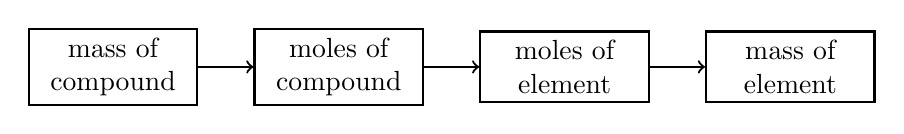
\begin{tikzpicture}[scale=0.70,every
			node/.style={draw,align=center,text width=0.75in,thick}]
			\node(masscomp) {mass of compound};
			\draw[thick,->] (masscomp.east) -- ++(1,0) node[at end,right](molcomp) {moles of compound};
			\draw[thick,->] (molcomp.east) -- ++(1,0) node[at end,right](molel) {moles of element};
			\draw[thick,->] (molel.east) -- ++(1,0) node[at end,right](massel) {mass of element};
		\end{tikzpicture}
	\end{center}

	\note<1>{
		\begin{tabularx}{\linewidth} {X X X}
			\bfseries Given & \bfseries Plan & \bfseries Find \\ \midrule
			\SI{25}{\gram}~\ch{CF2Cl2} &
			$\frac{\SI{1}{\mole}~\ch{CF2Cl2}}{\SI{2}{\mole}~\ch{Cl}}$
			& \si{\gram}~\ch{Cl}
		\end{tabularx}

		\begin{align*}
			\frac{\SI{25}{\gram}~\ch{CF2Cl2}}{1} \times
			\frac{\SI{1}{\mole}~\ch{CF2Cl2}}{\SI{120.91}{\gram}~\ch{CF2Cl2}}
			\times
			\frac{\SI{2}{\mole}~\ch{Cl}}{\SI{1}{\mole}~\ch{CF2Cl2}}
			\times
			\frac{\SI{35.453}{\gram}~\ch{Cl}}{\SI{1}{\mole}~\ch{Cl}}
			&= \SI{14.66}{\gram}~\ch{Cl} \\
			&= \boxed{\SI{15}{\gram}~\ch{Cl}}
		\end{align*}
	}
\end{inclass}

\begin{onyourown}
	Calculate the mass of arsenic in \SI{11}{\gram} of \ch{As(OH)3}
	(\SI{125.94}{\gram\per\mole}).
\end{onyourown}

\begin{frame}{Determining Chemical Composition Experimentally}
%	\begin{itemize}[<+->]
%		\item
	Recall the ``Gravimetric Analysis of Phosphorus in Fertilizer'' Lab %``Investigation of a Hydrate'' lab.
			\begin{itemize}
%				\item Heating the \ch{CuSO4 * $n$ H2O} caused
%					\ch{H2O} to evaporate:
%					\begin{reaction*}
%						CuSO4 * $n$ H2O\sld{} ->
%						CuSO4\sld{} + H2O\gas{}
%					\end{reaction*}
%				\item The difference in mass could be used to
%					calculate the \% water and value of $n$.
				\item Addition of \ch{NH3} and \ch{Mg^{2+}} caused \ch{MgNH4PO4 * 6 H2O} to precipitate:
					\begin{reaction*}
						6 H2O\lqd{} + MgHPO4\aq{} +
						NH3\aq{} ->
						MgNH4PO4 * 6 H2O\sld{}
					\end{reaction*}
				\item The mass of the product was proportional
					to the mass of the phosphorus in the
					fertilizer.
			\end{itemize}
			\pause

			\bigskip
%		\item 
			\mode<article>{\noindent}
			We can use a similar process for general composition
			analysis.
			\begin{itemize}
				\item We need to \alert{react} or
					\alert{decompose} a compound to smaller,
					measurable products.
				\item Weighing the products provides mole/mass
					ratios.
			\end{itemize}
	%\end{itemize}
\end{frame}

\begin{frame}{Combustion Analysis}
	Carbon-containing compounds, when burned, follow the general reaction:
	\begin{reaction*}
		C_{$x$}H_{$y$} + O2 -> CO2 + H2O \qquad \text{\footnotesize
		(unbalanced)}
	\end{reaction*}
	Measuring the mass of the produced \ch{CO2} and \ch{H2O} will allow for
	calculation of the original \alert{empirical formula}.
	\begin{center}
		\includegraphics[scale=0.4,trim={0 0 0 30pt},clip]{combustion.jpg}
	\end{center}
\end{frame}

\begin{inclass}
	Caproic acid contains only \ch{C}, \ch{H}, and \ch{O}. Combustion of
	\SI{0.450}{\gram} caproic acid gave \SI{0.418}{\gram} \ch{H2O} and
	\SI{1.02}{\gram} \ch{CO2}. What is the empirical formula of caproic
	acid?

	\vspace{\stretch{1}}

	\note{ \tiny
		\begin{tabularx}{\linewidth} {X X X}
			\bfseries Given & \bfseries Plan & \bfseries Find \\ \midrule
			\SI{0.418}{\gram} \ch{H2O} & $\frac{\SI{2}{\mole}~\ch{H}}{\SI{1}{\mole}~\ch{H2O}}$ & \si{\mole}~H \\
			\SI{1.02}{\gram} \ch{CO2}  & $\frac{\SI{1}{\mole}~\ch{C}}{\SI{1}{\mole}~\ch{CO2}}$ & \si{\mole}~C \\
			\SI{0.450}{\gram} caproic acid & & \si{\mole}~\ch{O}
		\end{tabularx}

		\begin{align*}
			\SI{0.418}{\gram}~\ch{H2O} \times \frac{\SI{1}{\mole}~\ch{H2O}}{\SI{18.0148}{\gram}~\ch{H2O}} \times \frac{\SI{2}{\mole}~\ch{H}}{\SI{1}{\mole}~\ch{H2O}} &= \SI{0.0464062882}{\mole}~\ch{H} \\
			\SI{1.02}{\gram}~\ch{CO2} \times \frac{\SI{1}{\mole}~\ch{CO2}}{\SI{44.009}{\gram}~\ch{CO2}} \times \frac{\SI{1}{\mole}~\ch{C}}{\SI{1}{\mole}~\ch{CO2}} &= \SI{0.0231770774}{\mole}~\ch{C} \\
			\shortintertext{How do we figure out oxygen?}
			\SI{0.04641}{\mole}~\ch{H} \times \frac{\SI{1.0079}{\gram}~\ch{H}}{\SI{1}{\mole}~\ch{H}}
			+ \SI{0.02318}{\mole}~\ch{C} \times \frac{\SI{12.011}{\gram}~\ch{C}}{\SI{1}{\mole}~\ch{C}} &= \SI{0.325152775}{\gram} \\
			\SI{0.450}{\gram} - \SI{0.32152775}{\gram} &= \SI{0.124847225}{\gram}~\ch{O} \\
			\SI{0.124847225}{\gram}~\ch{O} \times
			\frac{\SI{1}{\mole}~\ch{O}}{\SI{15.999}{\gram}~\ch{O}}
								   &=
								   \SI{0.007803439}{\mole}~\ch{O}
								   \\
			\ch{C}_{\frac{\num{0.0231770774}}{\num{0.007803439}}}\ch{H}_{\frac{\num{0.0464062882}}{\num{0.007803439}}}\ch{O}_{\frac{\num{0.007803439}}{\num{0.007803439}}}
			= \ch{C}_{2.97}\ch{H}_{5.95}\ch{O}_{1} &= \boxed{\ch{C3H6O}}
		\end{align*}
	}

	\pause

	What is the molecular formula if the molar mass of caproic acid is
	\SI{116.160}{\gram\per\mole?}

	\vspace{\stretch{1}}
\end{inclass}

\note{ \tiny
	\begin{tabular} {c c@{ $\times$ } c @{ @ }
		S[table-format=2.4,table-space-text-post=\,\si{\gram\per\mole}]<{\,\si{\gram\per\mole}} @{ $=$ }
	S[table-format=2.4]<{\,\si{\gram\per\mole}}}
		  & 3 & C & 12.011 & 36.033 \\
		  & 6 & H & 1.0079 & 6.0474 \\
		+ & 1 & O & 15.999 & 15.999 \\ \midrule
		\multicolumn{4}{c}{} & 58.0794
	\end{tabular}

	How many ``\ch{C3H6O}'' do we need to add up to \SI{116.160}{\gram\per\mole}?

	\begin{align*}
		\frac{\SI{116.160}{\gram\per\mole}}{\SI{58.0794}{\gram\per\mole}} &= 2 \\
		\therefore \ch{C}_{2 \times 3}\ch{H}_{2 \times 6}\ch{O}_{2 \times 1} &= \boxed{\ch{C6H12O2}}
	\end{align*}
	}

\clearpage

\begin{onyourown}
	Find the molecular formula of a \SI{1.50}{\gram} sample of an unknown
	hydrocarbon if it produces \SI{4.40}{\gram}~\ch{CO2} and
	\SI{2.70}{\gram}~\ch{H2O} after combustion. Assume the molar mass of
	this sample is \SI{64.17}{\gram\per\mole}.
\end{onyourown}

\begin{frame}{A Quick Intro to Organic Molecules}
	\only<+>{%
	\begin{description}
		\item[Organic:] Composed predominantly of carbon and hydrogen
		\item[Inorganic:] Everything else\ldots
	\end{description}
	}

	\only<+>{%
	Carbon is very versatile:
	\begin{itemize}
		\item C can bond to itself to form various structures:
			\begin{center}
				\includegraphics[scale=0.275]{carbon-to-itself.jpg}
			\end{center}
		\item C can form multiple bonds (including to itself):
			\begin{center}
				\includegraphics[scale=0.275]{multibond-carbon.jpg}
			\end{center}
	\end{itemize}
	Compounds containing \alert{only} carbon and hydrogen are called \alert{hydrocarbons}.
}

\mode<article>{\clearpage}

\only<+>{%
	\begin{center}
		\includegraphics[scale=0.45]{hydrocarbons.jpg}
	\end{center}
}
\end{frame}

\begin{frame}[t]{Another ``Combustion'' Example}
	\textbf{Chapter 4, Question 144}

	A particular coal contains \SI{2.55}{\percent} sulfur by mass. When the
	coal is burned, it produces \ch{SO2} emissions, which combine with
	rainwater to produce sulfuric acid. Use the formula of sulfuric acid to
	calculate the mass percent of \ch{S} in sulfuric acid. Then determine
	how much sulfuric acid is produced by the combustion of
	\SI{1.0e3}{\kilo\gram} of this coal.

	\mode<article>{\vspace*{20em}}

	\note{
		\begin{enumerate}
			\item We first need to calculate the calculate the
				molar mass of \ch{H2SO4}:
		\begin{tabular} {c c@{ $\times$ } c @{ @ }
			S[table-format=2.4,table-space-text-post=\,\si{\gram\per\mole}]<{\,\si{\gram\per\mole}} @{ $=$ }
		S[table-format=2.4]<{\,\si{\gram\per\mole}}}
			& 2 & H & 1.0079 & 2.0158 \\
			& 1 & S & 32.066 & 32.066 \\
			+ & 4 & O & 15.999 & 63.996 \\ \midrule
			\multicolumn{4}{c}{} & 98.0778
		\end{tabular}

	\item We can then figure out the mass percent of \ch{S} in \ch{H2SO4} as
		follows:
		\begin{align*}
			\frac{\SI{32.066}{\gram\per\mole}}{\SI{98.0778}{\gram\per\mole}} \times 100 &= \boxed{\SI{32.694}{\percent}} \\
			\intertext{\item This percentage will actually provide
				enough information to solve the problem without
			needing to go to moles:}
			\SI{1.0e3}{\kilo\gram}~\text{coal} \times \frac{\SI{2.55}{\kilo\gram}~\ch{S}}{\SI{100}{\kilo\gram}~\text{coal}} \times \frac{\SI{100}{\kilo\gram}~\ch{H2SO4}}{\SI{32.694}{\kilo\gram}~\ch{S}} &= \boxed{\SI{78}{\kilo\gram}}
		\end{align*}
\end{enumerate}
	}
\end{frame}

\mode<article>{\clearpage}

\begin{frame}[t]{Another Mass Percent Example}
	Vitamin C is composed of \SI{40.92}{\percent} \ch{C},
	\SI{4.68}{\percent} \ch{H}, and \SI{54.50}{\percent} \ch{O} by mass.
	The molecular weight of Vitamin C is known to be
	\SI{176.12}{\gram\per\mole}. Determine the empirical and molecular
	formula.

	\mode<article>{\vspace*{15em}}

	\note{We have a lot of percents, but no actual amount of sample.  Let's
		assume we have \SI{100}{\gram} of sample:
		\begin{center}
			\begin{math}
				\begin{array} {c
					@{~\times~\SI{100}{\gram}~\times~} c
				@{~=~} S[table-format=1.9]<{\,\si{\mole}}}
					\frac{\SI{40.92}{\gram}~\ch{C}}{\SI{100}{\gram}} & \frac{\SI{1}{\mole}~\ch{C}}{\SI{12.011}{\gram}} & 3.406877029 \\
					\frac{\SI{ 4.68}{\gram}~\ch{H}}{\SI{100}{\gram}} & \frac{\SI{1}{\mole}~\ch{H}}{\SI{1.0079}{\gram}} & 4.643317789 \\
					\frac{\SI{54.50}{\gram}~\ch{O}}{\SI{100}{\gram}} & \frac{\SI{1}{\mole}~\ch{O}}{\SI{15.999}{\gram}} & 3.406462904 \\
				\end{array}
				\end{math}
			\end{center}

			Now we have to find out relative amounts -- divide by the smallest \# moles:
				\begin{align*}
					\ch{C}_{\frac{3.406877029}{3.406462904}}\ch{H}_{\frac{3.406462904}{3.406462904}}\ch{O}_{\frac{4.643317789}{3.406462904}} &= \ch{C1H_{1.36}O1} \\
					\intertext{But these are not whole number ratios. We need to multiply by a factor that will provide whole numbers.}
					\ch{C}_{3 \times 1}\ch{H}_{3 \times 1.36}\ch{O}_{3 \times 1} &= \boxed{\ch{C3H4O3}}
				\end{align*}
			}
		\end{frame}
		\note{
			With a molar mass of \SI{176.12}{\gram\per\mole} and the mass of the empirical formula being \SI{88.0616}{\gram\per\mole}, we find that we need to multiply by 2:
				\begin{equation*}
					\frac{\SI{176.12}{\gram\per\mole}}{\SI{88.0616}{\gram\per\mole}} = 2 \therefore \boxed{\ch{C6H8O6}}
				\end{equation*}
		}

\end{document}
